Notes mostly based on \citet{maico2020categoria},
\citet{bradley2020topology}, \citet{borceux1994handbook}.

\section{Why study Category Theory}

The study of Category Theory enables us to view Mathematics from a vantage
point, and better understand how the different areas are connected. For example,
it might not always be clear which properties are \textit{topological}, and which aren't.
By looking at the subject from the distance (via Category Theory), we get
a glimpse at the connections (and disconnections) between different fields.

Another very interesting observation about Category Theory is that it's
becoming very popular in programming. This is highlighted for example
in the book \citet{milewski2018category}. In order to help
the understanding of the subject, I'll be using ``applications''
of Category Theory, mainly inspired by \citet{fong2019invitation}.
We'll also do coding examples using Catlab.jl, a Julia package
for applied Category Theory.

\section{Categories}

In this section, we formally define what a Category is, and we provide
some examples.

\subsection{Universes, Sets and Classes}

When working on Category Theory, it's common to find universal
statements such as ``for all topological spaces...''. The issue
with such statements is that, in a purely set-theoretical sense,
we have to know whether such large collection (``all topological spaces'')
is indeed a set. We might be tempted to say that's true, but
it's not so simple. The most known example of a possible failure of such
statements is Russel's Paradox of whether there is a set of all sets, for
which the answer is ``no''.

Therefore, in order to deal with such issue, we need a way to differentiate
between a valid set and an arbitrary collection. Here is where the notion of a Universe comes in.

\begin{definition}[Universe]
  We say that a set $\mathfrak U$ is a universe if\footnote{Definition from \citet{borceux1994handbook}}
  \begin{enumerate}[(i)]
    \item $x\in y$ and $ y\in \mathfrak U$, then $x \in \mathfrak U$;
    \item $I \in \mathfrak U$, and $\forall i \in I, x_i \in \mathfrak U$, then $\cup_{i\in I}x_i \in \mathfrak U$;
    \item $x \in \mathfrak U$ then $\mathcal P(x) \in \mathfrak U$, where $\mathcal P(x)$ is the power set;
    \item $x \in \mathfrak U$ and $f:x\to y$ is a surjective function, then $y \in \mathfrak U$;
    \item $\mathbb N \in \mathfrak U$.
  \end{enumerate}
\end{definition}

From this definition, one can prove the following proposition.
\begin{proposition}
  \begin{enumerate}[(i)]
    \item $x \in \mathfrak U$ and $y \subset x$, then $y \in \mathfrak U$;
    \item $x \in \mathfrak U$ and $y \subset x$, then $\{x,y\} \in \mathfrak U$;
    \item $x \in \mathfrak U$ and $y \subset x$, then $x\times y \in \mathfrak U$;
    \item $x \in \mathfrak U$ and $y \subset x$, then $y^x \in \mathfrak U$, where $y^x$ is the set of functions $f:x \to y$.
  \end{enumerate}
  \label{prop:universe}
\end{proposition}

With this definition, we state the axiom of existence universes.
\begin{axiom}
  Every set $S$ belongs to some universe $\mathfrak U$.
\end{axiom}

\begin{definition}
  For a fixed universe $\mathfrak U$, if a set $S$ is an element of $\mathfrak U$,
  then $S$ is called a \textit{small set}.
\end{definition}

Talking about ``small sets'' and ``big set'' might become daunting, so instead, we
use a different convention which is based on Gödel-Bernays theory of sets and classes.
This theory states that:
\begin{axiom}[Gödel-Bernays]
  Every set is a class, and a class is a set if and only if it belongs to some (other)
  class.
\end{axiom}

Note that using the notion of Universes, we can recover Gödel-Bernays theory. For that,
use the following definition:
\begin{definition}
  For a fixed universe $\mathfrak U$, we call $S$ a \textit{set} if it's an element
  of $\mathfrak U$, and call $S$ a \textit{class} if it's a subset of $\mathfrak U$.
  A class that is not a set is called a \textit{proper class}.
\end{definition}
Since every set is a class, if $S \in \mathfrak U$, then $S$ is a class,
since $U$ is a set and therefore a class, implying that $S$ belongs to a class.
On the other direction, if $S$ is a class and $S \in V \subset \mathfrak U$,
then since $V \subset \mathfrak U$, this means that $S \in \mathfrak U$, thus
it's a set.

From now on, whenever we say \textit{set} we are implying \textit{small set}
and whenever we say \textit{class} we are implying either small or big sets,
following \citet{borceux1994handbook} convention.


\subsection{What is a Category?}

Let's formally define a Category and provide some examples.

\begin{definition}[Category]
	A category $\mathcal C = \langle Ob_{\mathcal C}, Mor_{\mathcal C} \rangle$ consists
	of a class of objects $Ob_\mathcal C$ and a class of morphisms
	$Mor_\mathcal C$ satisfying the following conditions:
  \begin{enumerate}[(i)]
    \item Every morphism $f \in Mor_\mathcal C$ is associated to two objects $X,Y \in Ob_{\mathcal C}$
      which is represented by $f:X \to Y$ or $X \xrightarrow{\hspace{3mm}f \hspace{3mm}} Y$,
      where $dom(f) = X$ is called the domain of $f$ and $cod(f)=Y$ is the codomain. Moreover, we define
      $Mor_\mathcal C (X,Y)$ as 
      \begin{displaymath}
        Mor_\mathcal C (X,Y) := \{f \in Mor_\mathcal C \ : \ X \in dom(f), \ Y \in cod(f)\};
      \end{displaymath}
    \item For any three objects $X,Y, Z \in Ob_\mathcal C$, there exists a composition operator
      \begin{displaymath}
        \circ: Mor_\mathcal C (X,Y)   \times Mor_\mathcal C (Y,Z) \to Mor_\mathcal C (X,Z),
      \end{displaymath}
      \item For each object $X \in Ob_\mathcal C$ there exists a morfism $id_X \in Mor_\mathcal C (A,A)$
        called the identity.
  \end{enumerate}
  The composition operator must have the following properties:
  \begin{enumerate}[(p.1)]
    \item \textit{Associative}: for every $f \in Mor_\mathcal C (A,B),
      g \in Mor_\mathcal C (B,C), h \in Mor_\mathcal C (C,D)$ then
      \begin{displaymath}
        h \circ (g \circ f) = (h \circ g) \circ f.
      \end{displaymath}
    \item For any $f \in Mor_\mathcal C (X,Y)$, $g \in Mor_\mathcal C (Y,X)$, 
      \begin{displaymath}
        f \circ id_X = f,  \quad id_A \circ g = g.
      \end{displaymath}
  \end{enumerate}
\end{definition}

There are many ways to refers to the set of morphisms $Mor_\mathcal C (X,Y)$, such as
$\mathcal C(X,Y)$ or $\text{hom}_\mathcal C (X,Y)$. The reason for this is that
this set is sometimes called hom-set. In this notes, we'll use either $Mor_\mathcal C (X,Y)$
or $\mathcal C (X,Y)$ when there is no ambiguity. Also, we'll use $dom_f$ to mean $dom(f)$,
and similarly for the codomain.

Another point about conventions. When talking about composition, it's convenient
to use the operator $\fatsemi$, which is equivalent to the composition $\circ$,
but with the inverted order, i.e. $f \fatsemi g = g \circ f$. The convinience
will become clearer once we introduce Hasse diagrams as a way to represent Categories.

When the class of morphism $Mor_\mathcal C$ is a set, the category $\mathcal C$ is called
a \textit{locally small Category}. If both $Ob_\mathcal C$ and $Mor_\mathcal C$ are sets,
we then have a \textit{small Category}.

Finally, whenever it's not ambiguous, we might drop the subscript and use $Ob$
to refer to the objects of $\mathcal C$ and $Mor$ to refer to the morphisms of $\mathcal C$.

\subsection{Examples of Categories}

It's very common to represent Categories via Hasse Diagrams. In these diagrams, the
objects are represented as dots, and the morphisms as arrows. Let's show some examples.

\begin{example}[Category $\bm 1$]
  The Category $\bm 1$ consists of $Ob_{\bm 1} := \{a\}$ and $Mor_{\bm 1} = \{id_a\}$.
  The diagram for such Category is shown below.
  \begin{figure}[H]
    \begin{center}
      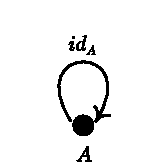
\includegraphics{./notebooks/1Cat}
    \end{center}
    \caption{Hasse diagram of Category $\bm 1$.}
    \label{fig:1Cat}
  \end{figure}
\end{example}

\begin{example}[Category $\bm 2$ and $\bm 3$]
  The Category $\bm 2$ consists of $Ob_{\bm 2} := \{a, b\}$ and $Mor_{\bm 1} = \{id_a, id_b, f\}$,
  where $f:a \to b$.
  The diagram for such Category is shown below.
  \begin{figure}[H]
    \begin{center}
      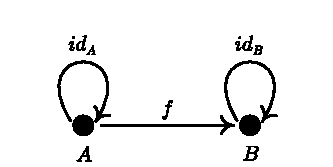
\includegraphics{./notebooks/2Cat}
    \end{center}
    \caption{Hasse diagram of Category $\bm 2$.}
    \label{fig:2Cat}
  \end{figure}

Since we know that identities are always present in Categories, we'll
omit them from future diagrams when there is no ambiguity. Thus,
the figure below represents the same diagram as Figure \ref{fig:2Cat}.
\begin{figure}[H]
  \begin{center}
    
\includegraphics{./notebooks/2Catsimple}
  \end{center}
  \caption{Hasse diagram of Category $\bm 2$ omitting identity morphisms.}
  \label{fig:2Catsimple}
\end{figure}

The Category $\bm 3$ has three morphisms besides the identities, given
by $f$, $g$ and their composition $f \fatsemi g$. The figure below
illustrates the Category with all it's morphisms.

\begin{figure}[H]
  \begin{center}
    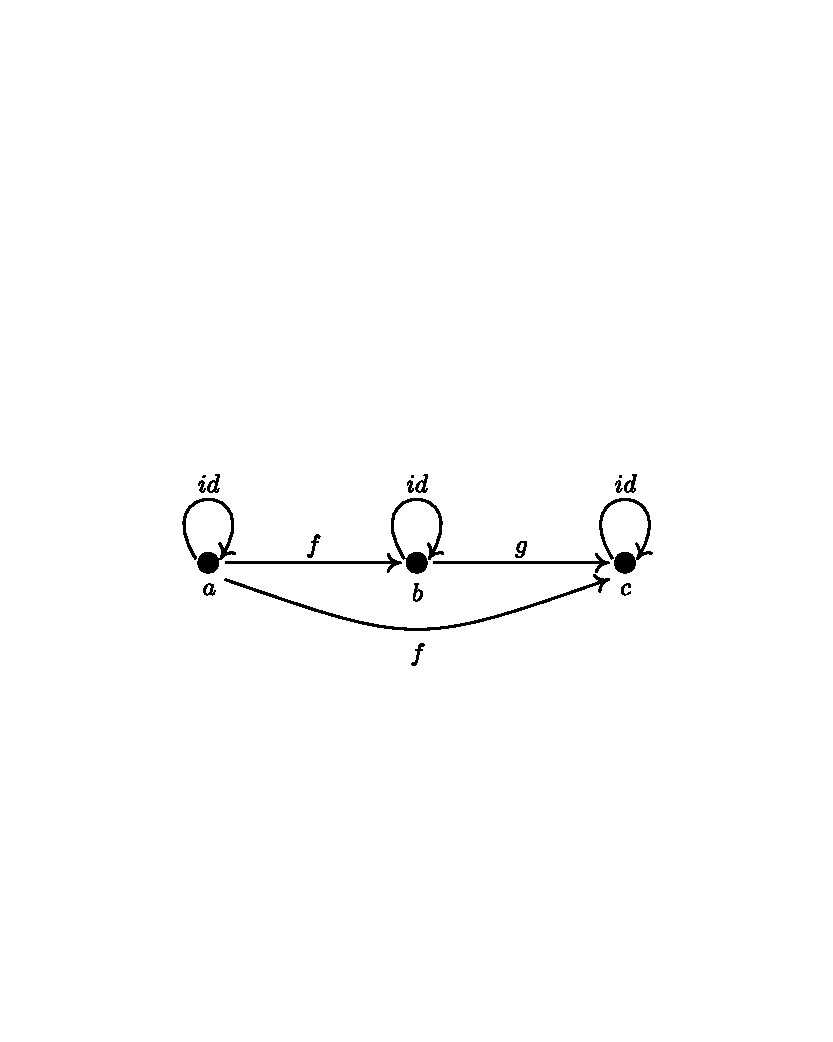
\includegraphics{./notebooks/3CatComplete}
  \end{center}
  \caption{Hasse diagram of Category $\bm 3$ showing all morphisms.}
  \label{fig:3Catcomplete}
\end{figure}

Drawing all the morphisms can make the diagram become too crowded, specially
as the number of objects and morphisms grows. Hence, we simplify the
diagram representation by ommiting not only the identity morphisms, but also
the compositions. These can always be assumed to exist, since they are a necessery
condition for every Category.
Thus, the figure below represents the same diagram as Figure \ref{fig:3Catcomplete}.

\begin{figure}[H]
  \begin{center}
    
\includegraphics{./notebooks/3Catsimple}
  \end{center}
  \caption{Hasse diagram of Category $\bm 3$ omitting identities and compositions.}
  \label{fig:3Catsimple}
\end{figure}

\end{example}

\begin{example}[Preorders]
  A Preorder is defined by a tuple $(P, \leq)$, where $P$ is a set of values, such that
  \begin{enumerate}[(i)]
    \item For $a,b \in P$, if $a\leq b$ and $b \leq c$, then $a \leq c$;
    \item For every $a \in P$, $a \leq a$.
  \end{enumerate}
  We can show that actually, this is a Category, which we'll call $\mathfrak P$,
  where $Ob_\mathfrak P = P$ and each morphism $f$ represents $a \leq b$, where
  $cod_f = a$ and $dom_f = b$.
  One example of preorder is the set of $\mathbb N$ equiped with the binary relation $\leq$
  which is shown in the diagram below.

\begin{figure}[H]
  \begin{center}
    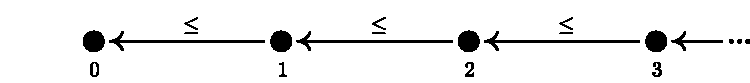
\includegraphics{./notebooks/NCat}
  \end{center}
  \caption{Hasse diagram of Preorder Category of Natural numbers.}
  \label{fig:NCat}
\end{figure}
\end{example}

Note that in preorders, there is at most one morphism between each pair of objects.
Thus, Categories with such property are often referred as \textit{thin Categories}
or \textit{preorder Category} (in \citet{fong2019invitation}, the authors call this
a \textit{preorder reflection}).

\subsection{Programming with Category Theory}

One might be surprised to find out that Category Theory,
although very abstract in nature, has actual applications in the
``real world''. A very interesting example of this is in programming.

In programming languages such as Julia, we can think of `Types`
as objects and functions as morphisms.

\subsection{Brief words on isomorphism}

A very important definition in Category Theory is the notion of isomorphism.
In Set Theory, we say that two sets are isomorphic if there is an invertible
function between them. Yet, this concept is not restricted to Set Theory
and can be generalized in Category Theory as follows:

\begin{definition}[Categorical Isomorphism]
  Let $\mathcal C$ be a category with $X,Y \in Ob_\mathcal C$ and $f \in Mor_\mathcal C (X,Y)$.
  \begin{enumerate}[(i)]
    \item We say that $f$ is \textit{left invertible} if there exists $g \in Mor_\mathcal C (Y,X)$ such
      that $g \circ f = id_X$;
    \item We say that $f$ is \textit{right invertible} if there exists $h \in Mor_\mathcal C (Y,X)$ such
      that $f \circ h = id_Y$;
    \item We say that $f$ is invertible if it's both left and right invertible.
  \end{enumerate}
  When an invertible morphism exists between $X$ and $Y$, we say that they are isomorphic.
\end{definition}
Note that when $f$ is invertible, the morphism that inverts $f$ is unique with the left and
right inverses coinciding, since
$g \circ id_Y = g \circ f \circ h = id_X \circ h = h$.


\section{Functors}

\begin{definition}[Functor]
  Let $\mathcal C$ and $\mathcal D$ be two Categories. A functor $F: \mathcal C \Rightarrow \mathcal D$ is
  a pair of mappings with the following properties:
  \begin{enumerate}[(i)]
    \item a mapping between objects
      \begin{displaymath}
        F:Ob_\mathcal C \to Ob_\mathcal D,
      \end{displaymath}
      where for each $A \in Ob_\mathcal C$, $F(A) \in Ob_\mathcal D$.
    \item a mapping between morphisms
      \begin{displaymath}
        F:Mor_\mathcal C \to Mor_\mathcal D,
      \end{displaymath}
      where there are two possibilities:
      \begin{enumerate}
        \item \textbf{Covariant Functor}, in which
          \begin{displaymath}
            F:Mor_\mathcal C(A,B) \to Mor_\mathcal D (F(A),F(B)),
          \end{displaymath}
          hence for a morphism $f:A \to B$, then $F(f):F(A) \to F(B)$.
        \item \textbf{Contravariant Functor}, in which
          \begin{displaymath}
            F:Mor_\mathcal C(A,B) \to Mor_\mathcal D (F(B),F(A)),
          \end{displaymath}
          hence for a morphism $f:A \to B$, then $F(f):F(B) \to F(A)$.
      \end{enumerate}
    \item Identities morphisms are preserved, i.e. for $A \in Ob_\mathcal C$
        \begin{displaymath}
          F(id_A) =  id_{F(A)}.
        \end{displaymath}
    \item Compositions are preserved, i.e. for $f \in Mor_\mathcal C(A,B)$
      and $ g \in Mor_\mathcal C(B,C)$,
      \begin{enumerate}
        \item For a \textbf{Covariant Functor},
          \begin{displaymath}
            F(f \circ g) = F(f) \circ F(g).
          \end{displaymath}
        \item For a \textbf{Contravariant Functor},
          \begin{displaymath}
            F(f \circ g) = F(g) \circ F(f).
          \end{displaymath}
      \end{enumerate}
  \end{enumerate}
  It's common for authors to refer to covariant functors only as functors, i.e.
  whenever someone say that $F$ is a functor, it might be implied that it's a covariant functor.
  We'll also use this convention whenever it's not ambiguous, and we'll always.
\end{definition}

